
\chapter{ORGANIZATION}
      \section{History}
      Before joining their bachelor's program, they were self-motivated, reading business model books and always focused on starting a company. In the 3rd year of their bachelor's degree, they started their own company with a vision to contribute to society by teaching trending topics in technologies rather than being a client-service organization. Driven by a passion for entrepreneurship, they actively hosted various tech occasions. Currently, they are excited about bioinformatics research.
      
      \section{Objectives}
      The company has the following objectives:
      \begin{itemize}
        \item Initial goal: Empowerment of the youths in entrepreneurship
        \item Convert to a corporate company
        \item Create events so that youth can showcase their talents
        \item Research in bioinformatics
      \end{itemize}

      \section{Working of Organization}
      \subsection{Input}

      \subsection{Output}
      The company provides the following services:
      \begin{itemize}
        \item Brand Guidaeline and Development
        \item Digital Marketing
        \item Event Management
        \item Technical Support for Business
        \item Cources on UTC(Urja Tech)
        \item Incubation and Enterpreneurship
        \item Human Resource Management
      \end{itemize}

      \section{Organizational Structure}
      The organizational structure of Urja Tech is hierarchical, characterized by multiple levels of management with a clear chain of command. This structure facilitates efficient supervision, decision-making, and accountability. Below is a detailed breakdown of the structure:
        \begin{enumerate}
           \item  \textbf{Top-Level Management}
            \begin{description}
                \item[\textbf{CEO:} ]  The CEO holds the highest authority within the company and is responsible for overall strategic planning, decision-making, and company oversight.
                
                \item \textbf{Directly Report to CEO:}
                
                \item[Legal Advisor: ]  The Legal Advisor handles all legal matters, ensuring compliance with laws and regulations. They provide legal advice to the CEO and other departments, manage legal risks, and oversee any legal proceedings involving the company.
                \item[Head Manager: ] The Head Manager oversees the company's daily operations and ensures the implementation of the CEO’s strategic plans. They coordinate between various departments, ensuring smooth workflow and operational efficiency.
                \item[CA(Chartered Accountant): ] The CA manages the financial operations of the company, including accounting, auditing, financial reporting, and budgeting. They ensure the financial health of the company and provide financial insights to support decision-making.
                 
            \end{description}
            
            \item \textbf{Middle Management}
            \begin{itemize}
                \item Under the \textbf{Head Manager:}
            \begin{description}
                \item[Manager: ] The Manager oversees specific operational areas or projects within the company. They ensure that their team meets performance targets and adheres to company policies.
                \item[System Admin: ] The System Admin manages the IT infrastructure, including system maintenance, network security, and technical support. They ensure that the company’s technology resources are efficient and secure.
                \item[HR (Human Resources) Manager:] The HR department handles recruitment, training, employee relations, and other HR functions. They ensure that the company attracts, retains, and develops the best talent.
            \end{description}
            \end{itemize}
            \item \textbf{Operational Level}
            \begin{itemize}
                \item Under the \textbf{Manager:}
            \begin{description}
                \item[Team Leader: ] The Team Leader supervises and guides a team of members, ensuring that tasks and projects are completed efficiently and effectively. They act as a bridge between the Manager and the team members.
            \end{description}
            \end{itemize}
            \item \textbf{Execution Level}
            \begin{itemize}
                \item Under the \textbf{Team Leader:}
            \begin{description}
                \item[Team Members:] Team Members carry out specific tasks and projects as directed by the Team Leader. They are responsible for the execution of the company’s day-to-day operations.
            \end{description}
            \end{itemize}
        \end{enumerate}
        \begin{figure}[H]
          
          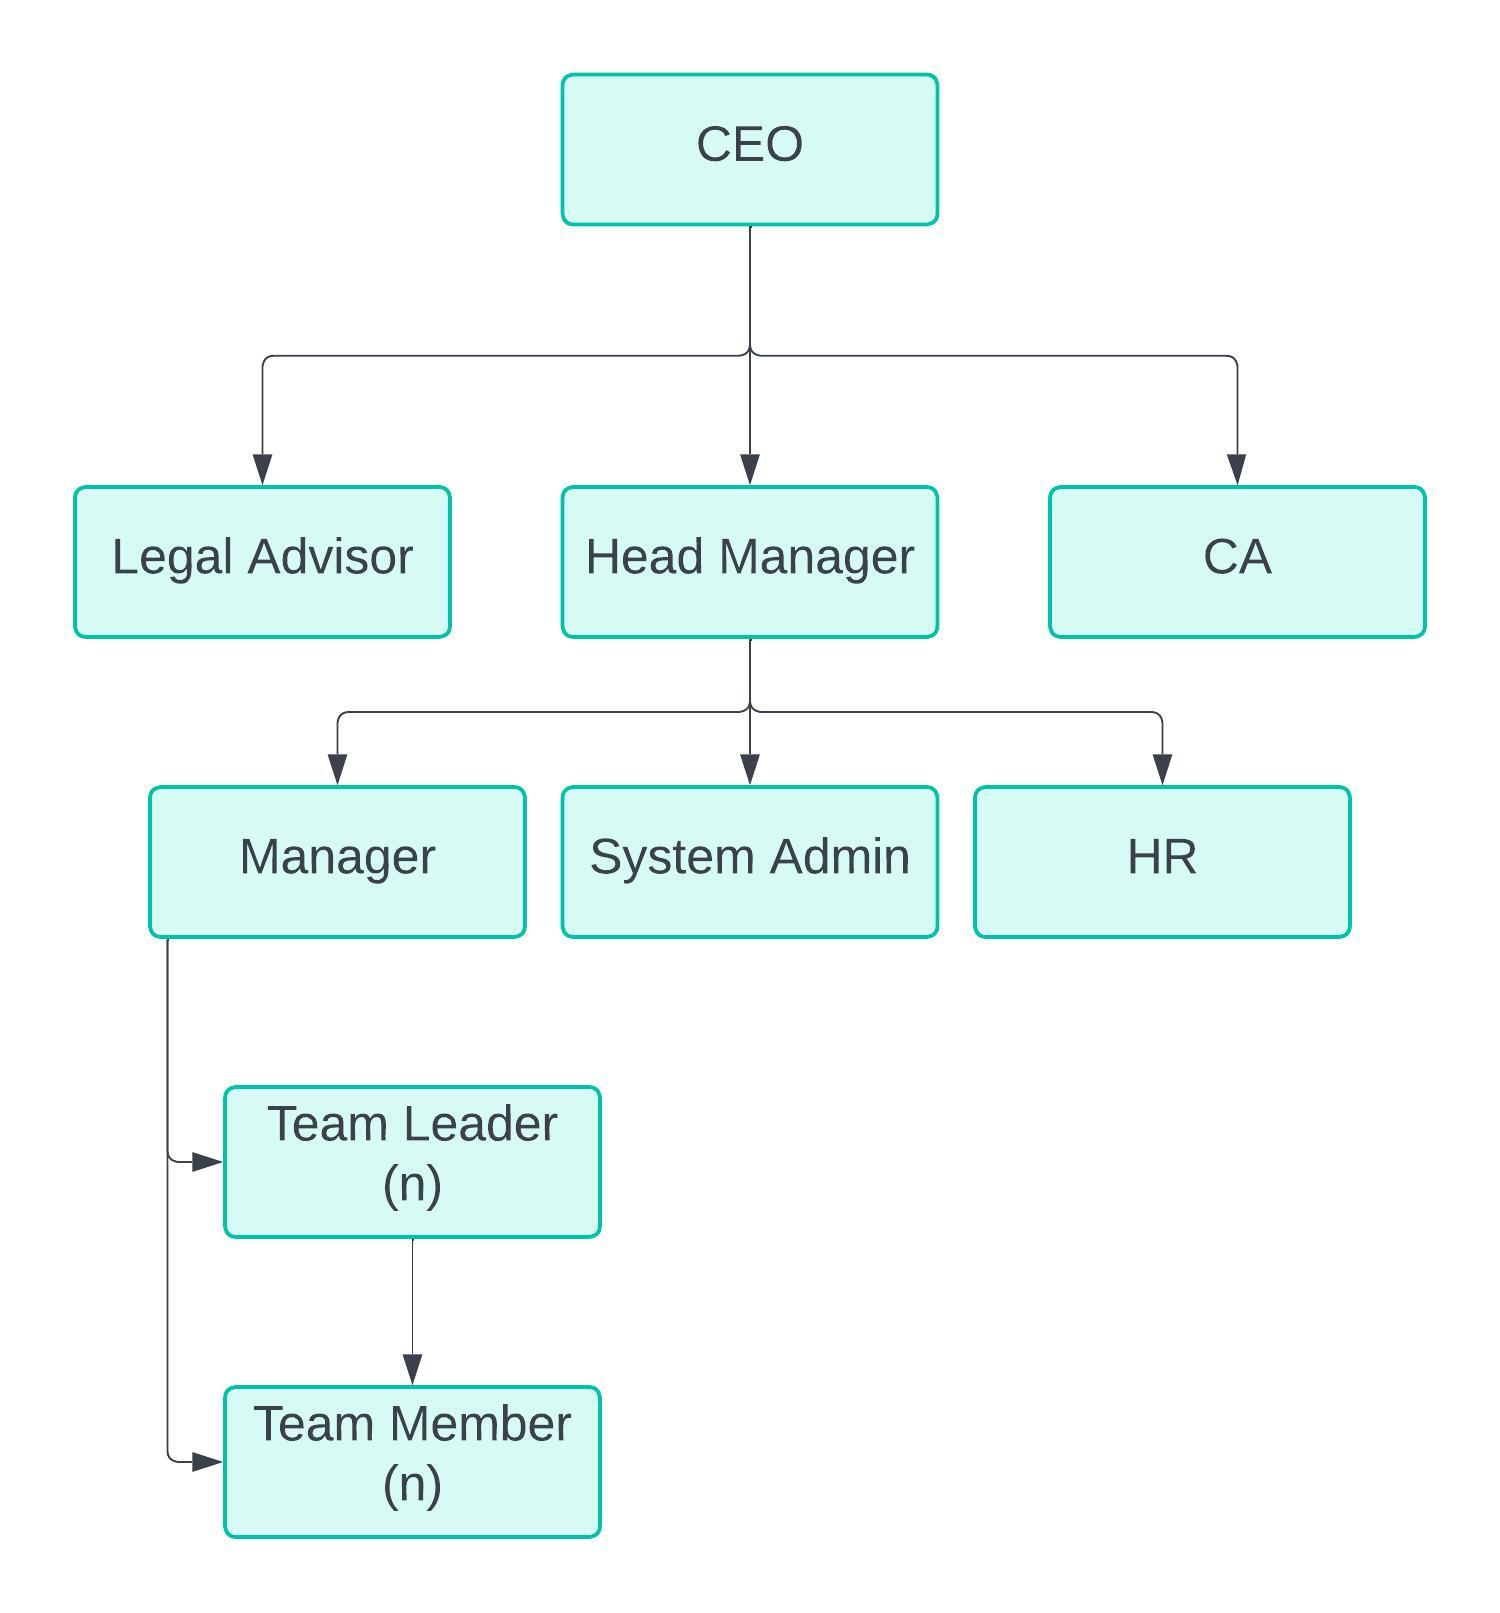
\includegraphics[width=\textwidth]{./Graphics/orgchart.jpeg}
          \caption{Organizational Structure of Urja Tech}
          \label{fig:orgchart}
        \end{figure}
        

      \section{Forms of Ownership}
      In the company, the CEO of the company is also the owner, making it a sole proprietorship. This business structure, where there is no legal distinction between the owner and the business entity, allows for complete control over all business decisions but also entails the risk of unlimited personal liability for the owner. Despite being a sole proprietorship, the company can still engage in partnerships with other businesses, including sister companies. Sister companies are separate legal entities that share common ownership or control, typically through a parent company. These partnerships can take various forms, such as strategic alliances, joint ventures, or contractual agreements, where each entity maintains its own separate legal and operational structure. In such a partnership, the sole proprietorship might collaborate with sister companies for various purposes, such as resource sharing, market expansion, cost reduction, or innovation. Each entity in the partnership retains its own legal identity, but they work together to leverage their combined strengths. The exact nature of these partnerships would depend on the agreements made between the companies and the strategic objectives they aim to achieve.
